\chapter{Background}

% A more extensive coverage of what's required to understand your
% work. In general you should assume the reader has a good undergraduate
% degree in computer science, but is not necessarily an expert in
% the particular area you've been working on. Hence this chapter
% may need to summarize some ``text book'' material.

% This is not something you'd normally require in an academic paper,
% and it may not be appropriate for your particular circumstances.
% Indeed, in some cases it's possible to cover all of the ``background''
% material either in the introduction or at appropriate places in
% the rest of the dissertation.

This chapter reviews background relevant to the remainder of this dissertaion.
The scope includes an overview of music theory and automatic composition
and also includes coverage of sequence probability models.

\section{A primer on Western music theory}

Music theory is a branch of musicology concerned with the study of the rules
and practices of music. While the general field includes study of acoustic
qualities such as timbre and waveform synthesis, our work is concerned with
modelling the musical composition itself rather than acoustic features. This is
justified because acoustic features are more closely related to a particular
reproduction (e.g. the skill of the performers, quality of the instruments) and
are likely to vary significantly across different performances. Indeed,
references to a piece of music generally refer to the underlying composition
itself rather than any particular performance of the piece. This suggests that
the composition itself is more significant and hence a more desirable modeling
target.

\subsection{Pitches, durations, and notes: the basic building blocks}

A \emph{note} is the most fundamental element of music and possesses two
primary attributes, a \emph{pitch} and a \emph{duration}. Though pitch is
closely related to physical frequency of vibration of a waveform (as measured
in Hertz), pitch its a perceptual property whose semantic meaning is derived
from a listener's perception. This distinction has been scrutinized by Terhardt
\cite{:/content/asa/journal/jasa/55/5/10.1121/1.1914648}, whose visual analogy
in \autoref{fig:pitch} illustrates how a pitch can be heard even if its
percieved frequency is absent just as one may see the word ``PITCH'' despite
being presented with only a suggestive shadow.

\begin{figure}[htpb]
    \centering
    
\includegraphics[width=0.6\linewidth]{Figures/pitch.pdf}
    \caption{Terhardt's visual analogy for pitch. Similar to how
        the viewer of this figure may percieve contours not present, pitch
        describes subjective information received by the listener even when
    physical frequencies are absent.}
    \label{fig:pitch}
\end{figure}

Despite its psychoacoustic nature, it is nevertheless useful to objectively
quantify pitch as a frequency. To do so, we first need some definitions. The
difference between two frequencies is called an \emph{interval} and an
\emph{octave} is an interval corresponding to the distance between a frequency
$f \in \RR^+$ and its doubling $2f$ or halving $f/2$. Two frequencies spaced
exactly an octave apart are perceived to be similar, suggesting that music is
percieved on a logarithmic scale.

Most Western music is based on the \emph{twelve-note chromatic scale}, which
divides an \emph{octave} into twelve distinct frequencies. The \emph{tuning
system} employed dictates the precise intervals between subdivisions, with
\emph{equal temperament tuning} (all subdivisions are equally spaced on a
logarithmic scale) presently the most widely used
method\cite{denton1997history}. \todo{Talk about well-tempered tuning and bach}
Under twelve-note equal temperament tuning, the distance between two
consecutive subdivisions ($1/12$ of an octave) is called a \emph{semitone}
(British) or \emph{half-step} (North American) and two semitones constitutes
a \emph{tone} or \emph{whole-step}.

When discussing music, \emph{note names} which enable succinct specification of
a musical pitch are often employed. In \emph{scientific pitch notation},
\emph{pitch classes} which represent a pitch modulo the octave are specified by
a letter ($C, D, E, F, G, A, B$) and optionally a single \emph{accidental}. Pitch
classes without accidentals are called \emph{natural} and correspond to the white
keys on a piano. Two accidentals are possible: sharps ($\#$) raise the natural
pitch class up one semitone and flats ($\flat$) lower by one semitone.
\autoref{fig:piano-keys} illustrates how these pitch classes map to keys on a
piano.

\begin{figure}[htpb]
    \centering
    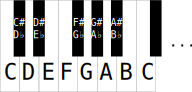
\includegraphics[width=0.6\linewidth]{Figures/piano-keys.pdf}
    \caption{Illustration of an octave in the 12-note chromatic scale
        on a piano keyboard.}
    \label{fig:piano-keys}
\end{figure}

Since pitch classes represent equivalence class of frequencies spaced an
integral number of octaves apart, unambiguously specifying a pitch requires not
only a pitch class but also an octave. In scientific pitch notation, this is
accomplished by appending an octave number to a pitch class letter (see
\autoref{fig:pitch-class}). Together, a pitch class and octave number uniquely
specify the notation for a pitch. On sheet music, the pitch of a note is
indicated by its vertical position with respect to the \emph{stave} (the five
horizontal lines and four spaces).

\begin{figure}[htpb]
    \centering
    \includegraphics[width=0.6\linewidth]{Figures/Pitch_notation.png}
    \caption{Scientific pitch notation and sheet music notation of $C$ notes at
    ten different octaves.  \todo{Cite wiki scientific pitch notation}}
    \label{fig:pitch-class}
\end{figure}

Note that the discussion of pitch thus far has not made any direct connection
between pitch and frequency. Indeed, this lack of dependence on absolute
physical frequency highlights music's \emph{transposition invariance property}:
many semantically relevant features in music are present the relative relations
between pitches rather than absolute frequencies and hence remain invariant
when the entire piece of music is offset by a constant frequency. However, a
fixed reference frequency is oftentimes required for performance and
reproduction purposes. To convert from pitch notation to physical frequencies,
common modern practice is to tune $A4$ to 440 Hz (a practice known as A440).

In addition to pitch, a note also possesses a \emph{duration}. The duration of
a note indicates how long it is to be played and is measured in fractions of a
\emph{whole note} (American) or \emph{semibreve} (British). Perhaps the most
common duration is a \emph{quarter-note} (American) or \emph{crotchet}
(British). Other note durations are also possible and the most common along
with their notation in sheet music are enumerated in
\autoref{fig:note-durations}. The relationship between durations and
physical time intervals is given by the \emph{tempo}, which is usually
denoted near the start of the piece in beats per minute.

\begin{figure}[htpb]
    \centering
    \includegraphics[width=0.6\linewidth]{Figures/note-durations.png}
    \caption{Comparison of various note durations. \todo{Cite wiki Whole note}}
    \label{fig:note-durations}
\end{figure}

Our work focuses in particular on \emph{tonal music}, a genre of music
characterized by the prevalence of one pitch class (the \emph{tonic}) around
which the melody and harmony are built.

A basic concept within tonal music is the \emph{scale}, which defines a subset
of pitch classes that are ``in key'' with respect to the tonic. Two fundamental
scales are the major (with step pattern
whole-whole-half-whole-whole-whole-half) and minor scales
(whole-half-whole-whole-half-whole-whole). The choice of tonic and scale is
collectively referred to as the \emph{key}. Many musical phenomena such as
stability, mood, expectation, and resolution can be attributed to choice of key
and \emph{modulations} (i.e. changes in key during the middle of a piece of
music).

\section{Neural sequence probability modeling}

Our work in later sections make heavy use of neural networks. In this section,
we briefly review the relevant concepts and set up notation.

\subsection{Neurons: the basic computation unit}

Neurons are the basic abstraction which are combined together to form
neural networks. A \emph{neuron} is a parametric model of a function $f : \RR^D \to
\RR$ from its $D$-dimensional input $\vec{x}$ to its output $y$. Our neurons will be
defined as
\begin{equation}
    f(\vec{x}) \coloneqq \sigma( \langle \vec{w}, \vec{x} \rangle)
\end{equation}
which can be viewed as an inner product with \emph{weights} $\vec{w}$ to
produce an \emph{activation} $z \coloneqq \langle \vec{w}, \vec{x} \rangle
\in \RR$ which is then squashed to a bounded domain by a non-linear
\textbf{activation function} $\sigma : \RR \to [L, U]$. This is visually
depicted in \autoref{fig:nn-single}, which also makes apparent the
interpretation of weight $w_i$ as the sensitivity of the output $y$ to the
input $x_i$.

\begin{figure}[htpb]
    \centering
    \input{Figures/nn-single.pdf_tex}
    \caption{A single neuron first computes an activation $z$ and then passes it through
    an activation function $\sigma(\cdot)$}
    \label{fig:nn-single}
\end{figure}

\subsection{Feedforward neural networks}

Multiple neurons may share inputs and have their outputs concatenated together
to form a \emph{layer} modelling a multivariate functions $f :
\RR^{D_\text{in}} \to \RR^{D_\text{out}}$. Multiple layers can then
be composed together to form a \emph{feedforwd neural network}.

\begin{figure}[htpb]
    \centering
    \input{Figures/nn-ffw.pdf_tex}
    \caption{Graph depiction of a feedforward neural network with $2$ hidden layers}
    \label{fig:nn-ffw}
\end{figure}

Although a single hidden layer is theoretically sufficient for a universal
function approximator\cite{Cybenko1993}, the number of hidden units to
guarantee reported theoretical bounds are usually unfeasibly large. Instead,
recent work in \emph{deep learning} has shown that deep models which contain
many hidden layers can achieve strong performance across a variety of
tasks\cite{Bengio2011}.

The improved modeling capacity gained by composing multiple layers is due to
the composition of multiple non-linear activation functions.
In fact, it is easy to show that removing activation functions would make
a deep network equivalent to a single matrix transform: let $\matr{W}_{l,l+1}$
denote the weights between layers $l$ and $l+1$. The original neural network
computes the function
\begin{equation}
    \sigma\left(
        \matr{W}_{L,L-1} \sigma \left(
            \matr{W}_{L-1,L-2}\cdots \sigma \left(
                \matr{W}_{2,1} \vec{x}
            \right) \cdots
        \right)
    \right)
\end{equation}
After removing the activation functions $\sigma$, we are left with
\begin{equation}
    \matr{W}_{L,L-1} \matr{W}_{L-1,L-2}\cdots \matr{W}_{2,1} \vec{x}
    = \vec{x}
    = \tilde{\matr{W}} \vec{x}
\end{equation}
where $\tilde{\matr{W}} = \left(\prod_{i=1}^{L-1} \matr{W}_{i,i+1} \right)$
is a matrix transform computing the same function as the neural network with
activation functions removed.

\subsection{Recurrent neural networks}

While feedforward neural networks provide a flexible model for approximating
arbitrary functions, they require a fixed-dimension input $\vec{x}$ and hence
cannot be applied to sequential data such as a sequence of notes. This shortcoming
motivates \emph{recurrent neural networks} (RNNs), which generalize feedforward
networks by introducing time-delayed connections between hidden layers (Elman
networks \cite{elman1990finding}) or from the output layers to the hidden layers (Jordan
networks \cite{jordan1997serial}). \autoref{fig:nn-rnn} illustrates a Elman-type network, which
\autoref{fig:rnn-elman} depicts as an equivalent network where the time-delayed
recurrent edges are redrawn as additional input nodes.

\begin{figure}[htpb]
    \centering
    \input{Figures/nn-rnn.pdf_tex}
    \caption{Graph depiction of an Elman-type RNN. Note the recurrent connections
    within the hidden layer.}
    \label{fig:nn-rnn}
\end{figure}

\begin{figure}[htpb]
    \centering
    \input{Figures/nn-rnn-elman.pdf_tex}
    \caption{Equivalent formulation of an Elman-type RNN treating the time-delayed hidden state
    as additional inputs to a feedforward network}
    \label{fig:rnn-elman}
\end{figure}


We can interpret the hidden layer as a temporal memory mechanism: the \emph{hidden
state} $\vec{h}_t$ is carried along throughout the computation and can be used
to store information from prior inputs for later use. One interpretation is to view
the hidden state $\vec{h}_t$ as an infinite-length prior context window, summarizing
all of the prior inputs into into a compact fixed-size vector.

This ability to
incorporate prior inputs into t wenables RNNs to excel at
sequence processing tasks, where the input sequence $X_n = (\vec{x}_t)_{1 \leq
t \leq T_n}$, $1 \leq n \leq N$, may have variable length $T_n$.

The time-delayed recurrent edges can be equivalently viewed as inputs to the
hidden nodes which are carried forward from the previous time step
(\autoref{fig:rnn-elman}).


This recursive structure can be unrolled
(\autoref{fig:rnn-multi-unrolled}) to yield a directed acyclic
\textbf{computation graph} containing nodes for the
\textbf{hidden state trajectory} $H_n = (\vec{h}_t)_{1 \leq t \leq T_n}$ and
\textbf{outputs} $Y_n = (\vec{y}_t)_{1 \leq t \leq T_n}$.

\begin{figure}[htpb]
    \centering
    \input{Figures/rnn-single-unrolled.pdf_tex}
    \caption{Signal flow diagram representation of a single-layer RNN and its corresponding
    expansion into a computation graph}
    \label{fig:rnn-single-unrolled}
\end{figure}

Just like feedforward networks, RNNs can be stacked by using the outputs of one
RNN as the inputs to another, forming \textbf{deep neural sequence models}. We
will describe multilayer RNNs as a dynamical system and use
$\matr{W}^{(l)}_{ij}$ to indicate the weight matrix relating variable $i$ to
variable $j$ at layer $l$. For example, \autoref{fig:rnn-multi-unrolled} is described
by the system of equations

\begin{eqnarray}
    \vec{h}^{(1)}_t &=& \matr{W}^{(1)}_{hx} \vec{x}^{(1)}_t + \matr{W}^{(1)}_{hh} \vec{h}^{(1)}_{t-1} \\
    \vec{y}^{(1)}_t &=& \matr{W}^{(1)}_{yh} \vec{h}^{(1)}_t \\
    \vec{x}^{(2)}_t &=& \vec{y}^{(1)}_t \\
    \vec{h}^{(2)}_t &=& \matr{W}^{(2)}_{hx} \vec{x}^{(2)}_t + \matr{W}^{(2)}_{hh} \vec{h}^{(1)}_{t-1} \\
    \vec{y}^{(2)}_t &=& \matr{W}^{(2)}_{yh} \vec{h}^{(2)}_t \\
\end{eqnarray}

\begin{figure}[htpb]
    \centering
    \input{Figures/rnn-multi-unrolled.pdf_tex}
    \caption{Unrolled computation graph for a 2-layer RNN}
    \label{fig:rnn-multi-unrolled}
\end{figure}

\subsubsection{Sequential processing and sampling}

We will train our RNNs to predict a distribution for the next character
$\vec{x}_{t+1}$ after the RNN has processed the sequence $\vec{x}_{1:t}$,
yielding a model which factorizes the sequence probability
\begin{equation}
    P(\vec{x}_{1:T}) = \prod_{t=1}^T P(\vec{x}_t | \vec{x}_{1:t-1} )
\end{equation}
Modeling this probability distribution over sequences is analogous to the
\textbf{language modeling} from speech recognition.

Note that the factorization of conditional distributions \emph{assumes a
sequential ordering in $t$}. This property is desirable as it enables sampling
from the model to generate new transcriptions by sampling from $P(\vec{x}_t |
\vec{x}_{1:t-1})$ at each timestep $t$ and using the sampled value as the next
input.

\todo{compare to bidirectional}.

\todo{for more details, see XYZ}.

\subsection{Parameter estimation of recursive neural networks}

\subsubsection{Modeling probabilities using the Boltzmann distribution and cross-entropy error criterion}

The parameters to the model are estimated in order to minimize the error
between the network outputs and provided labels. For language modeling, the
outputs $\vec{y}_t$ should parameterize a distribution for the next character
$P(\vec{x}_{t+1} | \vec{x}_{1:t})$. Suppose each input has finite support (i.e.
$\vec{x}_t \in [1,2,\cdots,K]$). If we choose the outputs to be $K$ dimensional
(i.e. $\vec{y}_t \in \RR^K$) then the \textbf{Boltzmann distribution}
(\autoref{eq:boltzmann-dist}) can be used:

\begin{equation}
    \label{eq:boltzmann-dist}
    P(\vec{x}_{t+1} = s | \vec{x}_{1:t})
    = \frac{\exp \left(-\vec{y}_{t,s}/T\right) }{ \sum_{k=1}^{K} \left(\exp -\vec{y}_{t,k}/T\right)}
\end{equation}

$T \in \RR^+$ is a \textbf{temperature} parameter \todo{relate to sampling}.

The labels provided are the actual next characters $\vec{x}_{t+1}$. Viewing
such labels as discrete probability distributions will all mass on a single atom,
one measure of difference between predictions and \todo{justify cross-entropy}

\subsubsection{Efficient graident computations through back-propogation}

Feed-forward neural networks are trained using back-propogation, an efficient
algorithm which consists of a forward pass to compute activations followed by
back-propogation of partial derivatives expanded according to the chain
rule\todo{cite backprop}. At the heart of back-propogation is the
\textbf{computation graph} of a a model: a directed acyclic graph where each
node represents a differentiable function that can compute its outputs and
Jacobian given inputs and activations\todo{cite theano}. By representing only
the dependencies between intermediate values, the sparsity imposed by the
computation graph enable back-propogation to ignore irrelevant
cross-derivatives and efficiently compute global gradients from local
computations.


Training of recursive neural networks is typically performed using
backpropogation through time (BPTT)\cite{at}, a technique computationally
equivalent to feedforward training of the unrolled computation graph. This is
easily seen: unrolling of a RNN yields a feed-forward structure where the
standard back-propogation algorithm applies.




\subsubsection{Vanishing gradients}

In practice, it is observed that the hidden state does not capture long range
dependencies well and tend to suffer from vanishing/exploding gradient during
training. LSTMs are an improved RNN architecture which solve both of these
problems by introducing gates on the inputs, hidden state, and outputs. GRUs are
a variation of LSTMs which ties the weights to the input and forget gates.

Vanishing/exploding gradients \cite{Bengio1994} are problems experienced by
RNNs arising from recursive applications of non-linear activations and linear dynamics
to the hidden state. To illustrate the vanishing gradient problem, consider
a simple recurrent network

\begin{eqnarray}
    h_t &=& \theta \phi(h_{t-1}) + \theta_x x_t \label{eq:ht-from-ht-1}\\
    y_t &=& \theta_y \phi(h_t)
\end{eqnarray}

After unrolling, the gradient of the error is given as a sum of the gradients
at each individual timestep

\begin{equation}
    \frac{\pd E}{\pd \theta} = \sum_{t=1}^S \frac{\pd E_t}{\pd \theta}
\end{equation}

Since the current hidden state $h_t$ depends on all prior hidden states $h_k$ ($k < t$),
the chain rule yields

\begin{equation}
    \frac{\pd E_t}{\pd \theta} = \sum_{k=1}^t \frac{\pd E_t}{\pd y_t} \frac{\pd y_t}{\pd h_t} \frac{\pd h_t}{\pd h_k} \frac{\pd h_k}{\pd \theta}
\end{equation}

Noting that time dynamics occur only through $h_t$

\begin{equation}
    \label{eq:prod-hi}
    \frac{\pd h_t}{\pd h_k} = \prod_{i=k+1}^t \frac{\pd h_i}{\pd h_{i-1}}
\end{equation}

The factors in the product can be obtained by differentiating \autoref{eq:ht-from-ht-1}

\begin{equation}
    \frac{\pd h_i}{\pd h_{i-1}} = \theta^\tp \diag\left[ \phi'(h_{i-1}) \right]
\end{equation}

Let $\|\cdot\|$ be any submultiplicative matrix norm. For illustration purposes, we will use the
\textbf{operator norm} defined as
\begin{equation}
    \| A \| = \sup_{x \in \RR^n; x \neq 0} \frac{|A x|}{|x|}
\end{equation}
where $|\cdot|$ is the standard Euclidian norm. However, any other submultiplicative norm
(e.g. Frobenius, spectral, nuclear, Shatten $p$-norms) is equally valid.

From submultiplicativity, we have

\begin{equation}
    \left\| \frac{\pd h_i}{\pd h_{i-1}} \right\|
    \leq \|\theta^\tp\| \| \diag\left[ \phi'(h_{i-1}) \right] \|
    \leq \gamma_{\theta} \gamma_\phi
\end{equation}

where $\gamma_\theta \coloneqq \|\theta\|$ is the norm of the hidden dynamics matrix $\theta$
and
\begin{align}
    \gamma_\phi
    &\coloneqq \sup_{h \in \RR^n} \| \diag \left[ \phi'(h) \right] \|  &\\
    &= \sup_{h \in \RR^n} \max_i \phi'(h)_i &\mbox{Operator norm of diag} \\
    &= \sup_{t \in \RR} \phi'(t) &\mbox{$\phi$ operates elementwise}
\end{align}

For common activation functions $\gamma_{\phi} \leq \infty$ (e.g. $\gamma_\phi = 1$ for $\phi = \tanh$
and $\gamma_\phi = 1/4$ for $\phi = \sigma$).

This gives a bound on \autoref{eq:prod-hi}, namely

\begin{equation}
    \left\| \frac{\pd h_t}{\pd h_k} \right\|
    = \left\| \prod_{i=k+1}^{t} \frac{\pd h_t}{\pd h_k} \right\|
    \leq (\gamma_\theta \gamma_\phi)^{t-k}
\end{equation}

When $|\gamma_\theta \gamma_\phi| < 1$, these gradients exponentially vanish to zero as
the time interval $t - k$ increases, hindering the network's ability to learn long-range
dynamics.

A similar argument \cite{Bengio1994} illustrates an analogous exponential explosion
when $\|\theta\| > 1$ (the ``exploding gradient'' problem).

The solution is to rewrite \autoref{eq:ht-from-ht-1} such that
\autoref{eq:prod-hi} does not vanish/explode for large $t - k$.
One possibility would be

\begin{equation}
    h_t = h_{t-1} + \theta_x x_t
\end{equation}

However, this solution is unsatisfactory as all hidden state dynamics have been
removed.

\subsubsection{Long Short Term Memory}

LSTMs are a RNN architecture which mitigates vanishing/exploding gradients by constraining
the hidden state dynamics. It does so by constraining the nonlinearity $\phi = \matr{I}$ to be the
identity and introducing three gates:
\begin{itemize}
    \item \textbf{Input gate}: scales input $x_t$ elementwise by $i_t \in [0,1]$, affects how $h_t$ is written to
    \item \textbf{Output gate}: scales output $y_t$ elementwise by $o_t \in [0,1]$, affects how $h_t$ is read from
    \item \textbf{Forget gate}: scales previous cell value $h_{t-1}$ by $f_t \in [0,1]$, acts as a reset mechanism
\end{itemize}

\begin{figure}[htpb]
    \centering
    \input{Figures/lstm-unit.pdf_tex}
    \caption{Single LSTM unit}
    \label{fig:lstm-unit}
\end{figure}

The equations for an LSTM are

\begin{eqnarray}
    i_t &=& \sigma(W_{xi} x_t + W_{yi} y_{t-1} + W_{ci} c_{t-1} + b_i) \\
    o_t &=& \sigma(W_{xo} x_t + W_{yo} y_{t-1} + W_{co} c_{t-1} + b_o) \\
    f_t &=& \sigma(W_{xf} x_t + W_{yf} y_{t-1} + W_{cf} c_{t-1} + b_f) \\
    h_t &=& f_t \odot h_{t-1} + i_t \odot \tanh(x_t W_{xc} + h_{t-1} W_{hc} + b_c) \label{eq:lstm-dynamics} \\
    y_t &=& o_t \odot \tanh(c_t)
\end{eqnarray}
where $\odot$ denotes elementwise multiplication of vectors.

Note that \autoref{eq:lstm-dynamics} has $\phi$ set to the identity function
hence $\gamma_\phi = 1$. This removal of the non-linearity in the hidden state
recursion is known as the \textbf{constant error carousel} \todo{cite}, which
allows the network to propogate errors without modification by $\varphi'(h_k)$.

The addition of the gates enables the model to learn when to read/write from
memory and when to reset, enabling longer-range dependencies to be learned when
an input is written to memory (i.e. $i_t$ high) and protected for a long
duration (i.e. $f_t \approx 1$ and $i_t \approx 0$).

Some authors define LSTMs such that $h_t$ is not used to compute gate activations,
referring to the case where $h_t$ is connected as ``peephole connections.'' In our
work, we use ``LSTM'' to refer to LSTMs with peephole connections.

LSTMs protect from vanishing gradient, but not exploding gradient. Research has shown
that gradient clipping is essential to permit successful applications \cite{Pascanu2012}.
